\documentclass[1p]{elsarticle_modified}
%\bibliographystyle{elsarticle-num}

%\usepackage[colorlinks]{hyperref}
%\usepackage{abbrmath_seonhwa} %\Abb, \Ascr, \Acal ,\Abf, \Afrak
\usepackage{amsfonts}
\usepackage{amssymb}
\usepackage{amsmath}
\usepackage{amsthm}
\usepackage{scalefnt}
\usepackage{amsbsy}
\usepackage{kotex}
\usepackage{caption}
\usepackage{subfig}
\usepackage{color}
\usepackage{graphicx}
\usepackage{xcolor} %% white, black, red, green, blue, cyan, magenta, yellow
\usepackage{float}
\usepackage{setspace}
\usepackage{hyperref}

\usepackage{tikz}
\usetikzlibrary{arrows}

\usepackage{multirow}
\usepackage{array} % fixed length table
\usepackage{hhline}

%%%%%%%%%%%%%%%%%%%%%
\makeatletter
\renewcommand*\env@matrix[1][\arraystretch]{%
	\edef\arraystretch{#1}%
	\hskip -\arraycolsep
	\let\@ifnextchar\new@ifnextchar
	\array{*\c@MaxMatrixCols c}}
\makeatother %https://tex.stackexchange.com/questions/14071/how-can-i-increase-the-line-spacing-in-a-matrix
%%%%%%%%%%%%%%%

\usepackage[normalem]{ulem}

\newcommand{\msout}[1]{\ifmmode\text{\sout{\ensuremath{#1}}}\else\sout{#1}\fi}
%SOURCE: \msout is \stkout macro in https://tex.stackexchange.com/questions/20609/strikeout-in-math-mode

\newcommand{\cancel}[1]{
	\ifmmode
	{\color{red}\msout{#1}}
	\else
	{\color{red}\sout{#1}}
	\fi
}

\newcommand{\add}[1]{
	{\color{blue}\uwave{#1}}
}

\newcommand{\replace}[2]{
	\ifmmode
	{\color{red}\msout{#1}}{\color{blue}\uwave{#2}}
	\else
	{\color{red}\sout{#1}}{\color{blue}\uwave{#2}}
	\fi
}

\newcommand{\Sol}{\mathcal{S}} %segment
\newcommand{\D}{D} %diagram
\newcommand{\A}{\mathcal{A}} %arc


%%%%%%%%%%%%%%%%%%%%%%%%%%%%%5 test

\def\sl{\operatorname{\textup{SL}}(2,\Cbb)}
\def\psl{\operatorname{\textup{PSL}}(2,\Cbb)}
\def\quan{\mkern 1mu \triangleright \mkern 1mu}

\theoremstyle{definition}
\newtheorem{thm}{Theorem}[section]
\newtheorem{prop}[thm]{Proposition}
\newtheorem{lem}[thm]{Lemma}
\newtheorem{ques}[thm]{Question}
\newtheorem{cor}[thm]{Corollary}
\newtheorem{defn}[thm]{Definition}
\newtheorem{exam}[thm]{Example}
\newtheorem{rmk}[thm]{Remark}
\newtheorem{alg}[thm]{Algorithm}

\newcommand{\I}{\sqrt{-1}}
\begin{document}

%\begin{frontmatter}
%
%\title{Boundary parabolic representations of knots up to 8 crossings}
%
%%% Group authors per affiliation:
%\author{Yunhi Cho} 
%\address{Department of Mathematics, University of Seoul, Seoul, Korea}
%\ead{yhcho@uos.ac.kr}
%
%
%\author{Seonhwa Kim} %\fnref{s_kim}}
%\address{Center for Geometry and Physics, Institute for Basic Science, Pohang, 37673, Korea}
%\ead{ryeona17@ibs.re.kr}
%
%\author{Hyuk Kim}
%\address{Department of Mathematical Sciences, Seoul National University, Seoul 08826, Korea}
%\ead{hyukkim@snu.ac.kr}
%
%\author{Seokbeom Yoon}
%\address{Department of Mathematical Sciences, Seoul National University, Seoul, 08826,  Korea}
%\ead{sbyoon15@snu.ac.kr}
%
%\begin{abstract}
%We find all boundary parabolic representation of knots up to 8 crossings.
%
%\end{abstract}
%\begin{keyword}
%    \MSC[2010] 57M25 
%\end{keyword}
%
%\end{frontmatter}

%\linenumbers
%\tableofcontents
%
\newcommand\colored[1]{\textcolor{white}{\rule[-0.35ex]{0.8em}{1.4ex}}\kern-0.8em\color{red} #1}%
%\newcommand\colored[1]{\textcolor{white}{ #1}\kern-2.17ex	\textcolor{white}{ #1}\kern-1.81ex	\textcolor{white}{ #1}\kern-2.15ex\color{red}#1	}

{\Large $\underline{12n_{0838}~(K12n_{0838})}$}

\setlength{\tabcolsep}{10pt}
\renewcommand{\arraystretch}{1.6}
\vspace{1cm}\begin{tabular}{m{100pt}>{\centering\arraybackslash}m{274pt}}
\multirow{5}{120pt}{
	\centering
	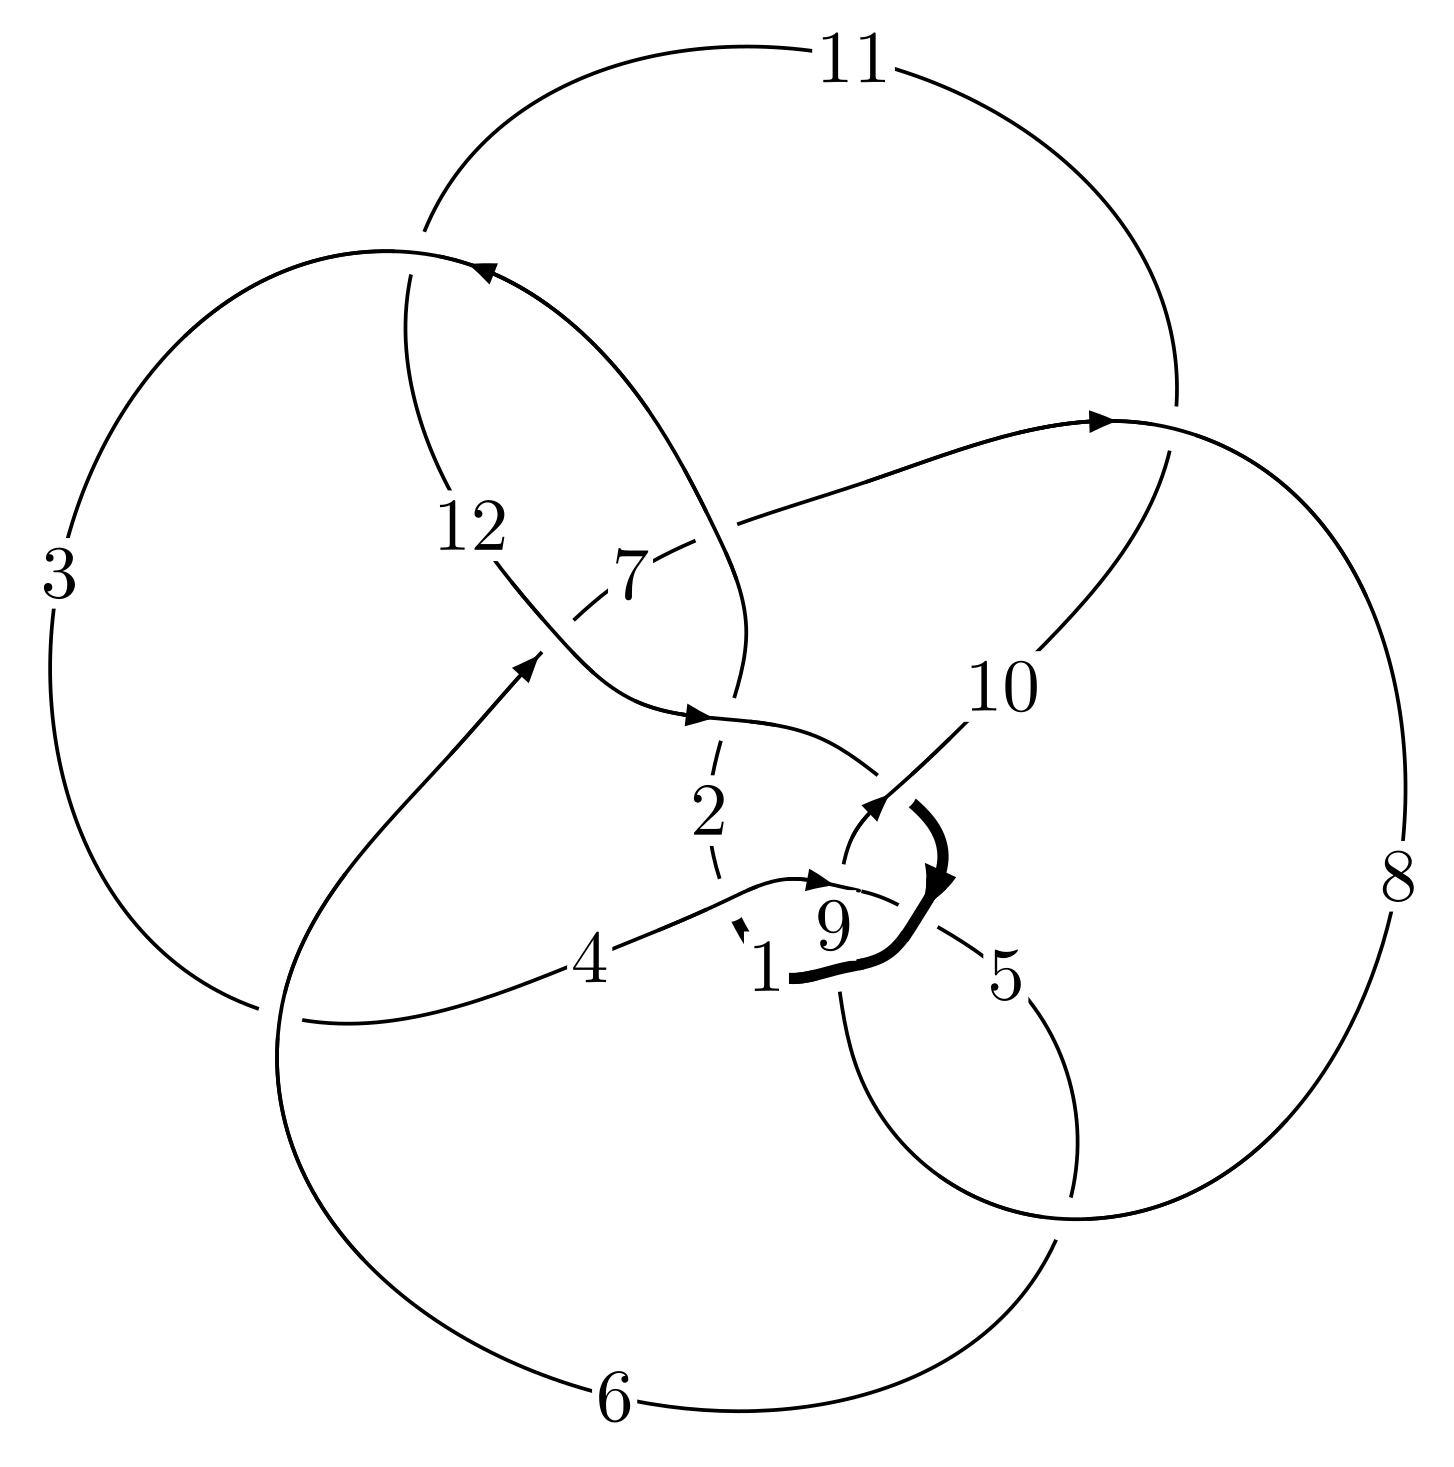
\includegraphics[width=112pt]{../../../GIT/diagram.site/Diagrams/png/2927_12n_0838.png}\\
\ \ \ A knot diagram\footnotemark}&
\allowdisplaybreaks
\textbf{Linearized knot diagam} \\
\cline{2-2}
 &
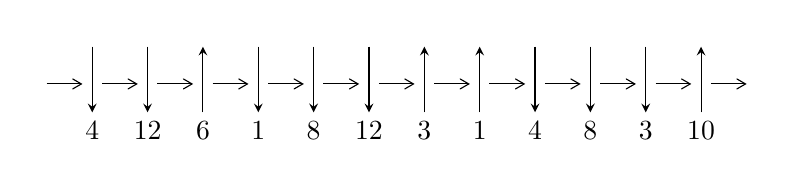
\begin{tikzpicture}[x=20pt, y=17pt]
	% nodes
	\node (C0) at (0, 0) {};
	\node (C1) at (1, 0) {};
	\node (C1U) at (1, +1) {};
	\node (C1D) at (1, -1) {4};

	\node (C2) at (2, 0) {};
	\node (C2U) at (2, +1) {};
	\node (C2D) at (2, -1) {12};

	\node (C3) at (3, 0) {};
	\node (C3U) at (3, +1) {};
	\node (C3D) at (3, -1) {6};

	\node (C4) at (4, 0) {};
	\node (C4U) at (4, +1) {};
	\node (C4D) at (4, -1) {1};

	\node (C5) at (5, 0) {};
	\node (C5U) at (5, +1) {};
	\node (C5D) at (5, -1) {8};

	\node (C6) at (6, 0) {};
	\node (C6U) at (6, +1) {};
	\node (C6D) at (6, -1) {12};

	\node (C7) at (7, 0) {};
	\node (C7U) at (7, +1) {};
	\node (C7D) at (7, -1) {3};

	\node (C8) at (8, 0) {};
	\node (C8U) at (8, +1) {};
	\node (C8D) at (8, -1) {1};

	\node (C9) at (9, 0) {};
	\node (C9U) at (9, +1) {};
	\node (C9D) at (9, -1) {4};

	\node (C10) at (10, 0) {};
	\node (C10U) at (10, +1) {};
	\node (C10D) at (10, -1) {8};

	\node (C11) at (11, 0) {};
	\node (C11U) at (11, +1) {};
	\node (C11D) at (11, -1) {3};

	\node (C12) at (12, 0) {};
	\node (C12U) at (12, +1) {};
	\node (C12D) at (12, -1) {10};
	\node (C13) at (13, 0) {};

	% arrows
	\draw[->,>={angle 60}]
	(C0) edge (C1) (C1) edge (C2) (C2) edge (C3) (C3) edge (C4) (C4) edge (C5) (C5) edge (C6) (C6) edge (C7) (C7) edge (C8) (C8) edge (C9) (C9) edge (C10) (C10) edge (C11) (C11) edge (C12) (C12) edge (C13) ;	\draw[->,>=stealth]
	(C1U) edge (C1D) (C2U) edge (C2D) (C3D) edge (C3U) (C4U) edge (C4D) (C5U) edge (C5D) (C6U) edge (C6D) (C7D) edge (C7U) (C8D) edge (C8U) (C9U) edge (C9D) (C10U) edge (C10D) (C11U) edge (C11D) (C12D) edge (C12U) ;
	\end{tikzpicture} \\
\hhline{~~} \\& 
\textbf{Solving Sequence} \\ \cline{2-2} 
 &
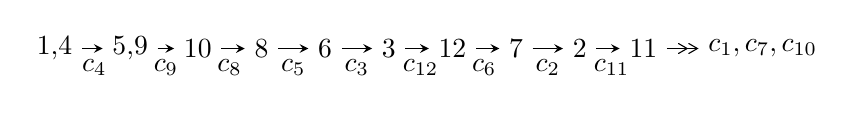
\begin{tikzpicture}[x=23pt, y=7pt]
	% node
	\node (A0) at (-1/8, 0) {1,4};
	\node (A1) at (17/16, 0) {5,9};
	\node (A2) at (17/8, 0) {10};
	\node (A3) at (25/8, 0) {8};
	\node (A4) at (33/8, 0) {6};
	\node (A5) at (41/8, 0) {3};
	\node (A6) at (49/8, 0) {12};
	\node (A7) at (57/8, 0) {7};
	\node (A8) at (65/8, 0) {2};
	\node (A9) at (73/8, 0) {11};
	\node (C1) at (1/2, -1) {$c_{4}$};
	\node (C2) at (13/8, -1) {$c_{9}$};
	\node (C3) at (21/8, -1) {$c_{8}$};
	\node (C4) at (29/8, -1) {$c_{5}$};
	\node (C5) at (37/8, -1) {$c_{3}$};
	\node (C6) at (45/8, -1) {$c_{12}$};
	\node (C7) at (53/8, -1) {$c_{6}$};
	\node (C8) at (61/8, -1) {$c_{2}$};
	\node (C9) at (69/8, -1) {$c_{11}$};
	\node (A10) at (11, 0) {$c_{1},c_{7},c_{10}$};

	% edge
	\draw[->,>=stealth]	
	(A0) edge (A1) (A1) edge (A2) (A2) edge (A3) (A3) edge (A4) (A4) edge (A5) (A5) edge (A6) (A6) edge (A7) (A7) edge (A8) (A8) edge (A9) ;
	\draw[->>,>={angle 60}]	
	(A9) edge (A10);
\end{tikzpicture} \\ 

\end{tabular} \\

\footnotetext{
The image of knot diagram is generated by the software ``\textbf{Draw programme}" developed by Andrew Bartholomew(\url{http://www.layer8.co.uk/maths/draw/index.htm\#Running-draw}), where we modified some parts for our purpose(\url{https://github.com/CATsTAILs/LinksPainter}).
}\phantom \\ \newline 
\centering \textbf{Ideals for irreducible components\footnotemark of $X_{\text{par}}$} 
 
\begin{align*}
I^u_{1}&=\langle 
b- u,\;-2 u^3+u^2+3 a-10 u-1,\;u^4+4 u^2+3 u+1\rangle \\
I^u_{2}&=\langle 
b+u,\;- u^5-3 u^3+u^2+2 a+3 u-2,\;u^6+4 u^4- u^3+2 u^2+u+1\rangle \\
I^u_{3}&=\langle 
-25 u^7+373 u^6-939 u^5+3197 u^4-5553 u^3+8389 u^2+2846 b-5460 u+4816,\\
\phantom{I^u_{3}}&\phantom{= \langle  }306 u^7+1468 u^6-1769 u^5+14032 u^4-19745 u^3+37228 u^2+36998 a-6881 u+6624,\\
\phantom{I^u_{3}}&\phantom{= \langle  }u^8-2 u^7+11 u^6-16 u^5+43 u^4-34 u^3+70 u^2-12 u+52\rangle \\
I^u_{4}&=\langle 
b+u,\;u^2+a+1,\;u^4+2 u^2+u+1\rangle \\
I^u_{5}&=\langle 
b- u,\;11 u^9+7 u^8+80 u^7+17 u^6+144 u^5-42 u^4+13 u^3-51 u^2+4 a+22 u-13,\\
\phantom{I^u_{5}}&\phantom{= \langle  }u^{10}+7 u^8-3 u^7+13 u^6-12 u^5+5 u^4-6 u^3+5 u^2-3 u+1\rangle \\
I^u_{6}&=\langle 
b+u+1,\;a+1,\;u^2+u+1\rangle \\
I^u_{7}&=\langle 
b+u+1,\;a+u,\;u^2+u+1\rangle \\
I^u_{8}&=\langle 
b- u+1,\;3 a-2 u+2,\;u^2- u+3\rangle \\
I^u_{9}&=\langle 
b+u-1,\;a,\;u^2- u+1\rangle \\
I^u_{10}&=\langle 
b,\;a-1,\;u^2+u+1\rangle \\
\\
I^v_{1}&=\langle 
a,\;b^2- b+1,\;v-1\rangle \\
\end{align*}
\raggedright * 11 irreducible components of $\dim_{\mathbb{C}}=0$, with total 44 representations.\\
\footnotetext{All coefficients of polynomials are rational numbers. But the coefficients are sometimes approximated in decimal forms when there is not enough margin.}
\newpage
\renewcommand{\arraystretch}{1}
\centering \section*{I. $I^u_{1}= \langle b- u,\;-2 u^3+u^2+3 a-10 u-1,\;u^4+4 u^2+3 u+1 \rangle$}
\flushleft \textbf{(i) Arc colorings}\\
\begin{tabular}{m{7pt} m{180pt} m{7pt} m{180pt} }
\flushright $a_{1}=$&$\begin{pmatrix}0\\u\end{pmatrix}$ \\
\flushright $a_{4}=$&$\begin{pmatrix}1\\0\end{pmatrix}$ \\
\flushright $a_{5}=$&$\begin{pmatrix}1\\u^2\end{pmatrix}$ \\
\flushright $a_{9}=$&$\begin{pmatrix}\frac{2}{3} u^3-\frac{1}{3} u^2+\frac{10}{3} u+\frac{1}{3}\\u\end{pmatrix}$ \\
\flushright $a_{10}=$&$\begin{pmatrix}\frac{2}{3} u^3-\frac{1}{3} u^2+\frac{7}{3} u+\frac{1}{3}\\u\end{pmatrix}$ \\
\flushright $a_{8}=$&$\begin{pmatrix}\frac{2}{3} u^3-\frac{1}{3} u^2+\frac{10}{3} u+\frac{1}{3}\\\frac{2}{3} u^3-\frac{1}{3} u^2+\frac{4}{3} u+\frac{1}{3}\end{pmatrix}$ \\
\flushright $a_{6}=$&$\begin{pmatrix}-\frac{1}{3} u^3+\frac{2}{3} u^2-\frac{5}{3} u+\frac{1}{3}\\-\frac{1}{3} u^3-\frac{1}{3} u^2-\frac{5}{3} u-\frac{2}{3}\end{pmatrix}$ \\
\flushright $a_{3}=$&$\begin{pmatrix}-\frac{1}{3} u^3+\frac{2}{3} u^2-\frac{2}{3} u+\frac{1}{3}\\\frac{1}{3} u^3-\frac{2}{3} u^2-\frac{1}{3} u-\frac{1}{3}\end{pmatrix}$ \\
\flushright $a_{12}=$&$\begin{pmatrix}-\frac{1}{3} u^3-\frac{1}{3} u^2-\frac{2}{3} u-\frac{2}{3}\\\frac{1}{3} u^3+\frac{1}{3} u^2+\frac{2}{3} u-\frac{1}{3}\end{pmatrix}$ \\
\flushright $a_{7}=$&$\begin{pmatrix}-\frac{2}{3} u^3+\frac{4}{3} u^2-\frac{4}{3} u+\frac{2}{3}\\- u^2-3 u-1\end{pmatrix}$ \\
\flushright $a_{2}=$&$\begin{pmatrix}- u\\u\end{pmatrix}$ \\
\flushright $a_{11}=$&$\begin{pmatrix}\frac{1}{3} u^3+\frac{1}{3} u^2+\frac{2}{3} u-\frac{1}{3}\\-\frac{1}{3} u^3-\frac{4}{3} u^2-\frac{2}{3} u-\frac{2}{3}\end{pmatrix}$\\&\end{tabular}
\flushleft \textbf{(ii) Obstruction class $= -1$}\\~\\
\flushleft \textbf{(iii) Cusp Shapes $= -\frac{16}{3} u^3+\frac{2}{3} u^2-\frac{56}{3} u-\frac{41}{3}$}\\~\\
\newpage\renewcommand{\arraystretch}{1}
\flushleft \textbf{(iv) u-Polynomials at the component}\newline \\
\begin{tabular}{m{50pt}|m{274pt}}
Crossings & \hspace{64pt}u-Polynomials at each crossing \\
\hline $$\begin{aligned}c_{1},c_{2},c_{4}\\c_{5},c_{6},c_{9}\\c_{10},c_{11}\end{aligned}$$&$\begin{aligned}
&u^4+4 u^2+3 u+1
\end{aligned}$\\
\hline $$\begin{aligned}c_{3},c_{12}\end{aligned}$$&$\begin{aligned}
&u^4+3 u^3+4 u^2+1
\end{aligned}$\\
\hline $$\begin{aligned}c_{7},c_{8}\end{aligned}$$&$\begin{aligned}
&u^4-5 u^3+7 u^2-3 u+3
\end{aligned}$\\
\hline
\end{tabular}\\~\\
\newpage\renewcommand{\arraystretch}{1}
\flushleft \textbf{(v) Riley Polynomials at the component}\newline \\
\begin{tabular}{m{50pt}|m{274pt}}
Crossings & \hspace{64pt}Riley Polynomials at each crossing \\
\hline $$\begin{aligned}c_{1},c_{2},c_{4}\\c_{5},c_{6},c_{9}\\c_{10},c_{11}\end{aligned}$$&$\begin{aligned}
&y^4+8 y^3+18 y^2- y+1
\end{aligned}$\\
\hline $$\begin{aligned}c_{3},c_{12}\end{aligned}$$&$\begin{aligned}
&y^4- y^3+18 y^2+8 y+1
\end{aligned}$\\
\hline $$\begin{aligned}c_{7},c_{8}\end{aligned}$$&$\begin{aligned}
&y^4-11 y^3+25 y^2+33 y+9
\end{aligned}$\\
\hline
\end{tabular}\\~\\
\newpage\flushleft \textbf{(vi) Complex Volumes and Cusp Shapes}
$$\begin{array}{c|c|c}  
\text{Solutions to }I^u_{1}& \I (\text{vol} + \sqrt{-1}CS) & \text{Cusp shape}\\
 \hline 
\begin{aligned}
u &= -0.367893 + 0.310982 I \\
a &= -0.86789 + 1.17701 I \\
b &= -0.367893 + 0.310982 I\end{aligned}
 & -0.650203 + 1.076870 I & -7.07727 - 6.47057 I \\ \hline\begin{aligned}
u &= -0.367893 - 0.310982 I \\
a &= -0.86789 - 1.17701 I \\
b &= -0.367893 - 0.310982 I\end{aligned}
 & -0.650203 - 1.076870 I & -7.07727 + 6.47057 I \\ \hline\begin{aligned}
u &= \phantom{-}0.36789 + 2.04303 I \\
a &= -0.132107 + 1.177010 I \\
b &= \phantom{-}0.36789 + 2.04303 I\end{aligned}
 & -15.7991 - 11.1024 I & \phantom{-}1.07727 + 3.92173 I \\ \hline\begin{aligned}
u &= \phantom{-}0.36789 - 2.04303 I \\
a &= -0.132107 - 1.177010 I \\
b &= \phantom{-}0.36789 - 2.04303 I\end{aligned}
 & -15.7991 + 11.1024 I & \phantom{-}1.07727 - 3.92173 I\\
 \hline 
 \end{array}$$\newpage\newpage\renewcommand{\arraystretch}{1}
\centering \section*{II. $I^u_{2}= \langle b+u,\;- u^5-3 u^3+u^2+2 a+3 u-2,\;u^6+4 u^4- u^3+2 u^2+u+1 \rangle$}
\flushleft \textbf{(i) Arc colorings}\\
\begin{tabular}{m{7pt} m{180pt} m{7pt} m{180pt} }
\flushright $a_{1}=$&$\begin{pmatrix}0\\u\end{pmatrix}$ \\
\flushright $a_{4}=$&$\begin{pmatrix}1\\0\end{pmatrix}$ \\
\flushright $a_{5}=$&$\begin{pmatrix}1\\u^2\end{pmatrix}$ \\
\flushright $a_{9}=$&$\begin{pmatrix}\frac{1}{2} u^5+\frac{3}{2} u^3-\frac{1}{2} u^2-\frac{3}{2} u+1\\- u\end{pmatrix}$ \\
\flushright $a_{10}=$&$\begin{pmatrix}\frac{1}{2} u^5+\frac{3}{2} u^3-\frac{1}{2} u^2-\frac{1}{2} u+1\\- u\end{pmatrix}$ \\
\flushright $a_{8}=$&$\begin{pmatrix}\frac{1}{2} u^5+\frac{3}{2} u^3-\frac{1}{2} u^2-\frac{3}{2} u+1\\-\frac{1}{2} u^5-\frac{5}{2} u^3+\frac{1}{2} u^2-\frac{3}{2} u\end{pmatrix}$ \\
\flushright $a_{6}=$&$\begin{pmatrix}\frac{1}{2} u^4+\frac{5}{2} u^2-\frac{1}{2} u+\frac{3}{2}\\\frac{1}{2} u^4+\frac{3}{2} u^2-\frac{1}{2} u-\frac{1}{2}\end{pmatrix}$ \\
\flushright $a_{3}=$&$\begin{pmatrix}-\frac{1}{4} u^5-\frac{1}{4} u^4+\cdots-\frac{3}{2} u-\frac{3}{4}\\-\frac{1}{4} u^5-\frac{3}{4} u^4+\cdots-\frac{5}{2} u^2-\frac{1}{4}\end{pmatrix}$ \\
\flushright $a_{12}=$&$\begin{pmatrix}-\frac{1}{4} u^5+\frac{1}{4} u^4+\cdots- u+\frac{3}{4}\\-\frac{1}{2} u^5-\frac{3}{2} u^3+\frac{1}{2} u^2+\frac{1}{2} u\end{pmatrix}$ \\
\flushright $a_{7}=$&$\begin{pmatrix}\frac{1}{4} u^5+\frac{3}{4} u^4+\cdots+\frac{7}{2} u^2+\frac{9}{4}\\\frac{1}{4} u^5+\frac{5}{4} u^4+\cdots+\frac{1}{2} u-\frac{1}{4}\end{pmatrix}$ \\
\flushright $a_{2}=$&$\begin{pmatrix}- u\\u\end{pmatrix}$ \\
\flushright $a_{11}=$&$\begin{pmatrix}\frac{3}{4} u^5+\frac{3}{4} u^4+\cdots-\frac{1}{2} u+\frac{1}{4}\\\frac{1}{2} u^5+\frac{3}{2} u^3-\frac{3}{2} u^2-\frac{3}{2} u-1\end{pmatrix}$\\&\end{tabular}
\flushleft \textbf{(ii) Obstruction class $= 1$}\\~\\
\flushleft \textbf{(iii) Cusp Shapes $= \frac{1}{4} u^5+\frac{3}{4} u^4+\frac{9}{4} u^3+\frac{7}{2} u^2+2 u+\frac{5}{4}$}\\~\\
\newpage\renewcommand{\arraystretch}{1}
\flushleft \textbf{(iv) u-Polynomials at the component}\newline \\
\begin{tabular}{m{50pt}|m{274pt}}
Crossings & \hspace{64pt}u-Polynomials at each crossing \\
\hline $$\begin{aligned}c_{1},c_{5},c_{6}\\c_{11}\end{aligned}$$&$\begin{aligned}
&u^6+4 u^4+u^3+2 u^2- u+1
\end{aligned}$\\
\hline $$\begin{aligned}c_{2},c_{4},c_{9}\\c_{10}\end{aligned}$$&$\begin{aligned}
&u^6+4 u^4- u^3+2 u^2+u+1
\end{aligned}$\\
\hline $$\begin{aligned}c_{3}\end{aligned}$$&$\begin{aligned}
&u^6+3 u^5+3 u^4+u^3+u^2+u+1
\end{aligned}$\\
\hline $$\begin{aligned}c_{7}\end{aligned}$$&$\begin{aligned}
&u^6+5 u^5+10 u^4+13 u^3+12 u^2+10 u+13
\end{aligned}$\\
\hline $$\begin{aligned}c_{8}\end{aligned}$$&$\begin{aligned}
&u^6-5 u^5+10 u^4-13 u^3+12 u^2-10 u+13
\end{aligned}$\\
\hline $$\begin{aligned}c_{12}\end{aligned}$$&$\begin{aligned}
&u^6-3 u^5+3 u^4- u^3+u^2- u+1
\end{aligned}$\\
\hline
\end{tabular}\\~\\
\newpage\renewcommand{\arraystretch}{1}
\flushleft \textbf{(v) Riley Polynomials at the component}\newline \\
\begin{tabular}{m{50pt}|m{274pt}}
Crossings & \hspace{64pt}Riley Polynomials at each crossing \\
\hline $$\begin{aligned}c_{1},c_{2},c_{4}\\c_{5},c_{6},c_{9}\\c_{10},c_{11}\end{aligned}$$&$\begin{aligned}
&y^6+8 y^5+20 y^4+17 y^3+14 y^2+3 y+1
\end{aligned}$\\
\hline $$\begin{aligned}c_{3},c_{12}\end{aligned}$$&$\begin{aligned}
&y^6-3 y^5+5 y^4+y^3+5 y^2+y+1
\end{aligned}$\\
\hline $$\begin{aligned}c_{7},c_{8}\end{aligned}$$&$\begin{aligned}
&y^6-5 y^5-6 y^4-3 y^3+144 y^2+212 y+169
\end{aligned}$\\
\hline
\end{tabular}\\~\\
\newpage\flushleft \textbf{(vi) Complex Volumes and Cusp Shapes}
$$\begin{array}{c|c|c}  
\text{Solutions to }I^u_{2}& \I (\text{vol} + \sqrt{-1}CS) & \text{Cusp shape}\\
 \hline 
\begin{aligned}
u &= \phantom{-}0.531659 + 0.753297 I \\
a &= -0.76444 - 1.54585 I \\
b &= -0.531659 - 0.753297 I\end{aligned}
 & \phantom{-}9.81524 - 4.74950 I & -0.79071 + 4.27718 I \\ \hline\begin{aligned}
u &= \phantom{-}0.531659 - 0.753297 I \\
a &= -0.76444 + 1.54585 I \\
b &= -0.531659 + 0.753297 I\end{aligned}
 & \phantom{-}9.81524 + 4.74950 I & -0.79071 - 4.27718 I \\ \hline\begin{aligned}
u &= -0.341164 + 0.448642 I \\
a &= \phantom{-}1.80674 - 0.44864 I \\
b &= \phantom{-}0.341164 - 0.448642 I\end{aligned}
 & \phantom{-}0.108732\phantom{ +0.000000I} & \phantom{-}                -6
0.581412 + 0. 10   I\phantom{ +0.000000I} \\ \hline\begin{aligned}
u &= -0.341164 - 0.448642 I \\
a &= \phantom{-}1.80674 + 0.44864 I \\
b &= \phantom{-}0.341164 + 0.448642 I\end{aligned}
 & \phantom{-}0.108732\phantom{ +0.000000I} & \phantom{-}                -6
0.581412 + 0. 10   I\phantom{ +0.000000I} \\ \hline\begin{aligned}
u &= -0.19050 + 1.91484 I \\
a &= -0.042290 - 1.122290 I \\
b &= \phantom{-}0.19050 - 1.91484 I\end{aligned}
 & \phantom{-}9.81524 + 4.74950 I & -0.79071 - 4.27718 I \\ \hline\begin{aligned}
u &= -0.19050 - 1.91484 I \\
a &= -0.042290 + 1.122290 I \\
b &= \phantom{-}0.19050 + 1.91484 I\end{aligned}
 & \phantom{-}9.81524 - 4.74950 I & -0.79071 + 4.27718 I\\
 \hline 
 \end{array}$$\newpage\newpage\renewcommand{\arraystretch}{1}
\centering \section*{III. $I^u_{3}= \langle -25 u^7+373 u^6+\cdots+2846 b+4816,\;306 u^7+1468 u^6+\cdots+36998 a+6624,\;u^8-2 u^7+\cdots-12 u+52 \rangle$}
\flushleft \textbf{(i) Arc colorings}\\
\begin{tabular}{m{7pt} m{180pt} m{7pt} m{180pt} }
\flushright $a_{1}=$&$\begin{pmatrix}0\\u\end{pmatrix}$ \\
\flushright $a_{4}=$&$\begin{pmatrix}1\\0\end{pmatrix}$ \\
\flushright $a_{5}=$&$\begin{pmatrix}1\\u^2\end{pmatrix}$ \\
\flushright $a_{9}=$&$\begin{pmatrix}-0.00827072 u^{7}-0.0396778 u^{6}+\cdots+0.185983 u-0.179037\\0.00878426 u^{7}-0.131061 u^{6}+\cdots+1.91848 u-1.69220\end{pmatrix}$ \\
\flushright $a_{10}=$&$\begin{pmatrix}-0.0170550 u^{7}+0.0913833 u^{6}+\cdots-1.73250 u+1.51316\\0.00878426 u^{7}-0.131061 u^{6}+\cdots+1.91848 u-1.69220\end{pmatrix}$ \\
\flushright $a_{8}=$&$\begin{pmatrix}-0.00827072 u^{7}-0.0396778 u^{6}+\cdots+0.185983 u-0.179037\\0.0351370 u^{7}-0.0242446 u^{6}+\cdots+1.67393 u+1.23120\end{pmatrix}$ \\
\flushright $a_{6}=$&$\begin{pmatrix}0.0925050 u^{7}-0.268636 u^{6}+\cdots+3.35694 u-1.17401\\-0.0562193 u^{7}+0.138791 u^{6}+\cdots-0.278285 u-0.569923\end{pmatrix}$ \\
\flushright $a_{3}=$&$\begin{pmatrix}-0.0345424 u^{7}+0.0107573 u^{6}+\cdots-1.10560 u-2.92421\\-0.00878426 u^{7}+0.131061 u^{6}+\cdots-2.91848 u+3.69220\end{pmatrix}$ \\
\flushright $a_{12}=$&$\begin{pmatrix}-0.0255014 u^{7}+0.0443267 u^{6}+\cdots+1.61511 u-0.552030\\0.0101897 u^{7}-0.0720309 u^{6}+\cdots-1.37456 u-1.60295\end{pmatrix}$ \\
\flushright $a_{7}=$&$\begin{pmatrix}0.214593 u^{7}-0.333261 u^{6}+\cdots+5.11320 u+4.17471\\-0.131061 u^{7}-0.00456781 u^{6}+\cdots+2.57625 u-8.07238\end{pmatrix}$ \\
\flushright $a_{2}=$&$\begin{pmatrix}- u\\u\end{pmatrix}$ \\
\flushright $a_{11}=$&$\begin{pmatrix}-0.111844 u^{7}+0.264095 u^{6}+\cdots-4.98824 u+3.16714\\0.197119 u^{7}-0.221012 u^{6}+\cdots+3.65074 u+2.26704\end{pmatrix}$\\&\end{tabular}
\flushleft \textbf{(ii) Obstruction class $= -1$}\\~\\
\flushleft \textbf{(iii) Cusp Shapes $= \frac{3}{1423} u^7+\frac{126}{1423} u^6-\frac{115}{1423} u^5+\frac{584}{1423} u^4+\frac{211}{1423} u^3+\frac{644}{1423} u^2+\frac{2932}{1423} u+\frac{3748}{1423}$}\\~\\
\newpage\renewcommand{\arraystretch}{1}
\flushleft \textbf{(iv) u-Polynomials at the component}\newline \\
\begin{tabular}{m{50pt}|m{274pt}}
Crossings & \hspace{64pt}u-Polynomials at each crossing \\
\hline $$\begin{aligned}c_{1},c_{2},c_{4}\\c_{5},c_{6},c_{9}\\c_{10},c_{11}\end{aligned}$$&$\begin{aligned}
&u^8-2 u^7+11 u^6-16 u^5+43 u^4-34 u^3+70 u^2-12 u+52
\end{aligned}$\\
\hline $$\begin{aligned}c_{3},c_{12}\end{aligned}$$&$\begin{aligned}
&(u^4-3 u^2+2 u+5)^2
\end{aligned}$\\
\hline $$\begin{aligned}c_{7},c_{8}\end{aligned}$$&$\begin{aligned}
&(u^4+4 u^3+3 u^2+5)^2
\end{aligned}$\\
\hline
\end{tabular}\\~\\
\newpage\renewcommand{\arraystretch}{1}
\flushleft \textbf{(v) Riley Polynomials at the component}\newline \\
\begin{tabular}{m{50pt}|m{274pt}}
Crossings & \hspace{64pt}Riley Polynomials at each crossing \\
\hline $$\begin{aligned}c_{1},c_{2},c_{4}\\c_{5},c_{6},c_{9}\\c_{10},c_{11}\end{aligned}$$&$\begin{aligned}
&y^8+18 y^7+\cdots+7136 y+2704
\end{aligned}$\\
\hline $$\begin{aligned}c_{3},c_{12}\end{aligned}$$&$\begin{aligned}
&(y^4-6 y^3+19 y^2-34 y+25)^2
\end{aligned}$\\
\hline $$\begin{aligned}c_{7},c_{8}\end{aligned}$$&$\begin{aligned}
&(y^4-10 y^3+19 y^2+30 y+25)^2
\end{aligned}$\\
\hline
\end{tabular}\\~\\
\newpage\flushleft \textbf{(vi) Complex Volumes and Cusp Shapes}
$$\begin{array}{c|c|c}  
\text{Solutions to }I^u_{3}& \I (\text{vol} + \sqrt{-1}CS) & \text{Cusp shape}\\
 \hline 
\begin{aligned}
u &= -0.318348 + 0.988585 I \\
a &= \phantom{-}0.902055 + 0.085959 I \\
b &= \phantom{-}1.18274 + 1.38356 I\end{aligned}
 & \phantom{-}12.33700 - 3.66386 I & \phantom{-}2.00000 + 2.00000 I \\ \hline\begin{aligned}
u &= -0.318348 - 0.988585 I \\
a &= \phantom{-}0.902055 - 0.085959 I \\
b &= \phantom{-}1.18274 - 1.38356 I\end{aligned}
 & \phantom{-}12.33700 + 3.66386 I & \phantom{-}2.00000 - 2.00000 I \\ \hline\begin{aligned}
u &= \phantom{-}0.24810 + 1.76504 I \\
a &= \phantom{-}0.260593 - 1.307340 I \\
b &= -0.11249 - 2.13718 I\end{aligned}
 & \phantom{-}12.33700 - 3.66386 I & \phantom{-}2.00000 + 2.00000 I \\ \hline\begin{aligned}
u &= \phantom{-}0.24810 - 1.76504 I \\
a &= \phantom{-}0.260593 + 1.307340 I \\
b &= -0.11249 + 2.13718 I\end{aligned}
 & \phantom{-}12.33700 + 3.66386 I & \phantom{-}2.00000 - 2.00000 I \\ \hline\begin{aligned}
u &= \phantom{-}1.18274 + 1.38356 I \\
a &= \phantom{-}0.228120 + 0.463986 I \\
b &= -0.318348 + 0.988585 I\end{aligned}
 & \phantom{-}12.33700 - 3.66386 I & \phantom{-}2.00000 + 2.00000 I \\ \hline\begin{aligned}
u &= \phantom{-}1.18274 - 1.38356 I \\
a &= \phantom{-}0.228120 - 0.463986 I \\
b &= -0.318348 - 0.988585 I\end{aligned}
 & \phantom{-}12.33700 + 3.66386 I & \phantom{-}2.00000 - 2.00000 I \\ \hline\begin{aligned}
u &= -0.11249 + 2.13718 I \\
a &= -0.121537 - 1.103540 I \\
b &= \phantom{-}0.24810 - 1.76504 I\end{aligned}
 & \phantom{-}12.33700 + 3.66386 I & \phantom{-}2.00000 - 2.00000 I \\ \hline\begin{aligned}
u &= -0.11249 - 2.13718 I \\
a &= -0.121537 + 1.103540 I \\
b &= \phantom{-}0.24810 + 1.76504 I\end{aligned}
 & \phantom{-}12.33700 - 3.66386 I & \phantom{-}2.00000 + 2.00000 I\\
 \hline 
 \end{array}$$\newpage\newpage\renewcommand{\arraystretch}{1}
\centering \section*{IV. $I^u_{4}= \langle b+u,\;u^2+a+1,\;u^4+2 u^2+u+1 \rangle$}
\flushleft \textbf{(i) Arc colorings}\\
\begin{tabular}{m{7pt} m{180pt} m{7pt} m{180pt} }
\flushright $a_{1}=$&$\begin{pmatrix}0\\u\end{pmatrix}$ \\
\flushright $a_{4}=$&$\begin{pmatrix}1\\0\end{pmatrix}$ \\
\flushright $a_{5}=$&$\begin{pmatrix}1\\u^2\end{pmatrix}$ \\
\flushright $a_{9}=$&$\begin{pmatrix}- u^2-1\\- u\end{pmatrix}$ \\
\flushright $a_{10}=$&$\begin{pmatrix}- u^2+u-1\\- u\end{pmatrix}$ \\
\flushright $a_{8}=$&$\begin{pmatrix}- u^2-1\\u^2+1\end{pmatrix}$ \\
\flushright $a_{6}=$&$\begin{pmatrix}u^3+u+1\\- u^3+u^2- u\end{pmatrix}$ \\
\flushright $a_{3}=$&$\begin{pmatrix}- u^3-2 u+1\\u^3+u-1\end{pmatrix}$ \\
\flushright $a_{12}=$&$\begin{pmatrix}- u^3- u^2-2 u-2\\u^3+u^2+2 u+1\end{pmatrix}$ \\
\flushright $a_{7}=$&$\begin{pmatrix}2 u^3+2 u\\-2 u^3+u^2- u+1\end{pmatrix}$ \\
\flushright $a_{2}=$&$\begin{pmatrix}- u\\u\end{pmatrix}$ \\
\flushright $a_{11}=$&$\begin{pmatrix}- u^3- u^2-1\\u^3\end{pmatrix}$\\&\end{tabular}
\flushleft \textbf{(ii) Obstruction class $= 1$}\\~\\
\flushleft \textbf{(iii) Cusp Shapes $= -8 u^3+2 u^2-12 u-7$}\\~\\
\newpage\renewcommand{\arraystretch}{1}
\flushleft \textbf{(iv) u-Polynomials at the component}\newline \\
\begin{tabular}{m{50pt}|m{274pt}}
Crossings & \hspace{64pt}u-Polynomials at each crossing \\
\hline $$\begin{aligned}c_{1},c_{5},c_{6}\\c_{11}\end{aligned}$$&$\begin{aligned}
&u^4+2 u^2- u+1
\end{aligned}$\\
\hline $$\begin{aligned}c_{2},c_{4},c_{9}\\c_{10}\end{aligned}$$&$\begin{aligned}
&u^4+2 u^2+u+1
\end{aligned}$\\
\hline $$\begin{aligned}c_{3}\end{aligned}$$&$\begin{aligned}
&u^4+u^3+4 u^2+2 u+3
\end{aligned}$\\
\hline $$\begin{aligned}c_{7}\end{aligned}$$&$\begin{aligned}
&u^4+3 u^3+3 u^2+u+1
\end{aligned}$\\
\hline $$\begin{aligned}c_{8}\end{aligned}$$&$\begin{aligned}
&u^4-3 u^3+3 u^2- u+1
\end{aligned}$\\
\hline $$\begin{aligned}c_{12}\end{aligned}$$&$\begin{aligned}
&u^4- u^3+4 u^2-2 u+3
\end{aligned}$\\
\hline
\end{tabular}\\~\\
\newpage\renewcommand{\arraystretch}{1}
\flushleft \textbf{(v) Riley Polynomials at the component}\newline \\
\begin{tabular}{m{50pt}|m{274pt}}
Crossings & \hspace{64pt}Riley Polynomials at each crossing \\
\hline $$\begin{aligned}c_{1},c_{2},c_{4}\\c_{5},c_{6},c_{9}\\c_{10},c_{11}\end{aligned}$$&$\begin{aligned}
&y^4+4 y^3+6 y^2+3 y+1
\end{aligned}$\\
\hline $$\begin{aligned}c_{3},c_{12}\end{aligned}$$&$\begin{aligned}
&y^4+7 y^3+18 y^2+20 y+9
\end{aligned}$\\
\hline $$\begin{aligned}c_{7},c_{8}\end{aligned}$$&$\begin{aligned}
&y^4-3 y^3+5 y^2+5 y+1
\end{aligned}$\\
\hline
\end{tabular}\\~\\
\newpage\flushleft \textbf{(vi) Complex Volumes and Cusp Shapes}
$$\begin{array}{c|c|c}  
\text{Solutions to }I^u_{4}& \I (\text{vol} + \sqrt{-1}CS) & \text{Cusp shape}\\
 \hline 
\begin{aligned}
u &= -0.343815 + 0.625358 I \\
a &= -0.727136 + 0.430014 I \\
b &= \phantom{-}0.343815 - 0.625358 I\end{aligned}
 & -1.13814 + 3.38562 I & -6.32177 - 8.18198 I \\ \hline\begin{aligned}
u &= -0.343815 - 0.625358 I \\
a &= -0.727136 - 0.430014 I \\
b &= \phantom{-}0.343815 + 0.625358 I\end{aligned}
 & -1.13814 - 3.38562 I & -6.32177 + 8.18198 I \\ \hline\begin{aligned}
u &= \phantom{-}0.343815 + 1.358440 I \\
a &= \phantom{-}0.727136 - 0.934099 I \\
b &= -0.343815 - 1.358440 I\end{aligned}
 & \phantom{-}4.42801 - 2.37936 I & \phantom{-}0.32177 + 1.76734 I \\ \hline\begin{aligned}
u &= \phantom{-}0.343815 - 1.358440 I \\
a &= \phantom{-}0.727136 + 0.934099 I \\
b &= -0.343815 + 1.358440 I\end{aligned}
 & \phantom{-}4.42801 + 2.37936 I & \phantom{-}0.32177 - 1.76734 I\\
 \hline 
 \end{array}$$\newpage\newpage\renewcommand{\arraystretch}{1}
\centering \section*{V. $I^u_{5}= \langle b- u,\;11 u^9+7 u^8+\cdots+4 a-13,\;u^{10}+7 u^8+\cdots-3 u+1 \rangle$}
\flushleft \textbf{(i) Arc colorings}\\
\begin{tabular}{m{7pt} m{180pt} m{7pt} m{180pt} }
\flushright $a_{1}=$&$\begin{pmatrix}0\\u\end{pmatrix}$ \\
\flushright $a_{4}=$&$\begin{pmatrix}1\\0\end{pmatrix}$ \\
\flushright $a_{5}=$&$\begin{pmatrix}1\\u^2\end{pmatrix}$ \\
\flushright $a_{9}=$&$\begin{pmatrix}-\frac{11}{4} u^9-\frac{7}{4} u^8+\cdots-\frac{11}{2} u+\frac{13}{4}\\u\end{pmatrix}$ \\
\flushright $a_{10}=$&$\begin{pmatrix}-\frac{11}{4} u^9-\frac{7}{4} u^8+\cdots-\frac{13}{2} u+\frac{13}{4}\\u\end{pmatrix}$ \\
\flushright $a_{8}=$&$\begin{pmatrix}-\frac{11}{4} u^9-\frac{7}{4} u^8+\cdots-\frac{11}{2} u+\frac{13}{4}\\-\frac{3}{4} u^9-\frac{1}{4} u^8+\cdots-\frac{3}{2} u+\frac{7}{4}\end{pmatrix}$ \\
\flushright $a_{6}=$&$\begin{pmatrix}-\frac{7}{4} u^9-\frac{3}{4} u^8+\cdots-5 u+\frac{15}{4}\\-\frac{1}{4} u^9-\frac{1}{4} u^8+\cdots-\frac{1}{2} u+\frac{3}{4}\end{pmatrix}$ \\
\flushright $a_{3}=$&$\begin{pmatrix}-2 u^9- u^8+\cdots-\frac{9}{2} u+5\\-\frac{3}{4} u^9-\frac{1}{4} u^8+\cdots-\frac{3}{2} u+\frac{5}{4}\end{pmatrix}$ \\
\flushright $a_{12}=$&$\begin{pmatrix}\frac{7}{4} u^9+\frac{7}{4} u^8+\cdots+u-\frac{9}{4}\\\frac{3}{4} u^9+\frac{1}{4} u^8+\cdots+\frac{7}{2} u-\frac{7}{4}\end{pmatrix}$ \\
\flushright $a_{7}=$&$\begin{pmatrix}-\frac{15}{4} u^9-\frac{7}{4} u^8+\cdots-\frac{17}{2} u+\frac{35}{4}\\- u^9-\frac{1}{2} u^8+\cdots-3 u+2\end{pmatrix}$ \\
\flushright $a_{2}=$&$\begin{pmatrix}- u\\u\end{pmatrix}$ \\
\flushright $a_{11}=$&$\begin{pmatrix}-\frac{11}{2} u^9-\frac{7}{2} u^8+\cdots-\frac{29}{2} u+\frac{15}{2}\\-\frac{11}{4} u^9-\frac{7}{4} u^8+\cdots-5 u+\frac{15}{4}\end{pmatrix}$\\&\end{tabular}
\flushleft \textbf{(ii) Obstruction class $= -1$}\\~\\
\flushleft \textbf{(iii) Cusp Shapes $= -\frac{1}{4} u^9+\frac{3}{4} u^8- u^7+\frac{27}{4} u^6-\frac{1}{2} u^5+\frac{31}{2} u^4-\frac{11}{4} u^3+\frac{19}{4} u^2-\frac{15}{2} u-\frac{3}{4}$}\\~\\
\newpage\renewcommand{\arraystretch}{1}
\flushleft \textbf{(iv) u-Polynomials at the component}\newline \\
\begin{tabular}{m{50pt}|m{274pt}}
Crossings & \hspace{64pt}u-Polynomials at each crossing \\
\hline $$\begin{aligned}c_{1},c_{2},c_{4}\\c_{5},c_{6},c_{9}\\c_{10},c_{11}\end{aligned}$$&$\begin{aligned}
&u^{10}+7 u^8-3 u^7+13 u^6-12 u^5+5 u^4-6 u^3+5 u^2-3 u+1
\end{aligned}$\\
\hline $$\begin{aligned}c_{3},c_{12}\end{aligned}$$&$\begin{aligned}
&u^{10}+6 u^9+\cdots+8 u+4
\end{aligned}$\\
\hline $$\begin{aligned}c_{7},c_{8}\end{aligned}$$&$\begin{aligned}
&u^{10}-8 u^9+\cdots-34 u+4
\end{aligned}$\\
\hline
\end{tabular}\\~\\
\newpage\renewcommand{\arraystretch}{1}
\flushleft \textbf{(v) Riley Polynomials at the component}\newline \\
\begin{tabular}{m{50pt}|m{274pt}}
Crossings & \hspace{64pt}Riley Polynomials at each crossing \\
\hline $$\begin{aligned}c_{1},c_{2},c_{4}\\c_{5},c_{6},c_{9}\\c_{10},c_{11}\end{aligned}$$&$\begin{aligned}
&y^{10}+14 y^9+75 y^8+183 y^7+177 y^6+22 y^5+7 y^4-32 y^3- y^2+y+1
\end{aligned}$\\
\hline $$\begin{aligned}c_{3},c_{12}\end{aligned}$$&$\begin{aligned}
&y^{10}+2 y^9+\cdots+120 y+16
\end{aligned}$\\
\hline $$\begin{aligned}c_{7},c_{8}\end{aligned}$$&$\begin{aligned}
&y^{10}-20 y^9+\cdots-300 y+16
\end{aligned}$\\
\hline
\end{tabular}\\~\\
\newpage\flushleft \textbf{(vi) Complex Volumes and Cusp Shapes}
$$\begin{array}{c|c|c}  
\text{Solutions to }I^u_{5}& \I (\text{vol} + \sqrt{-1}CS) & \text{Cusp shape}\\
 \hline 
\begin{aligned}
u &= -0.486518 + 0.632836 I \\
a &= \phantom{-}0.079644 + 0.328409 I \\
b &= -0.486518 + 0.632836 I\end{aligned}
 & -0.61761 + 1.79087 I & -3.17008 - 3.84422 I \\ \hline\begin{aligned}
u &= -0.486518 - 0.632836 I \\
a &= \phantom{-}0.079644 - 0.328409 I \\
b &= -0.486518 - 0.632836 I\end{aligned}
 & -0.61761 - 1.79087 I & -3.17008 + 3.84422 I \\ \hline\begin{aligned}
u &= \phantom{-}0.621008 + 0.075641 I \\
a &= \phantom{-}1.79439 - 1.51840 I \\
b &= \phantom{-}0.621008 + 0.075641 I\end{aligned}
 & \phantom{-}9.12328 - 3.14851 I & -1.88527 + 0.97081 I \\ \hline\begin{aligned}
u &= \phantom{-}0.621008 - 0.075641 I \\
a &= \phantom{-}1.79439 + 1.51840 I \\
b &= \phantom{-}0.621008 - 0.075641 I\end{aligned}
 & \phantom{-}9.12328 + 3.14851 I & -1.88527 - 0.97081 I \\ \hline\begin{aligned}
u &= \phantom{-}0.239585 + 0.499962 I \\
a &= -1.76390 + 0.24899 I \\
b &= \phantom{-}0.239585 + 0.499962 I\end{aligned}
 & -0.61761 + 1.79087 I & -3.17008 - 3.84422 I \\ \hline\begin{aligned}
u &= \phantom{-}0.239585 - 0.499962 I \\
a &= -1.76390 - 0.24899 I \\
b &= \phantom{-}0.239585 - 0.499962 I\end{aligned}
 & -0.61761 - 1.79087 I & -3.17008 + 3.84422 I \\ \hline\begin{aligned}
u &= -0.06345 + 1.88716 I \\
a &= -0.084885 + 1.197580 I \\
b &= -0.06345 + 1.88716 I\end{aligned}
 & \phantom{-}9.12328 + 3.14851 I & -1.88527 - 0.97081 I \\ \hline\begin{aligned}
u &= -0.06345 - 1.88716 I \\
a &= -0.084885 - 1.197580 I \\
b &= -0.06345 - 1.88716 I\end{aligned}
 & \phantom{-}9.12328 - 3.14851 I & -1.88527 + 0.97081 I \\ \hline\begin{aligned}
u &= -0.31062 + 1.88752 I \\
a &= \phantom{-}0.474749 + 1.077290 I \\
b &= -0.31062 + 1.88752 I\end{aligned}
 & -17.0114\phantom{ +0.000000I} & \phantom{-}                -6
1.110699 + 0. 10   I\phantom{ +0.000000I} \\ \hline\begin{aligned}
u &= -0.31062 - 1.88752 I \\
a &= \phantom{-}0.474749 - 1.077290 I \\
b &= -0.31062 - 1.88752 I\end{aligned}
 & -17.0114\phantom{ +0.000000I} & \phantom{-}                -6
1.110699 + 0. 10   I\phantom{ +0.000000I}\\
 \hline 
 \end{array}$$\newpage\newpage\renewcommand{\arraystretch}{1}
\centering \section*{VI. $I^u_{6}= \langle b+u+1,\;a+1,\;u^2+u+1 \rangle$}
\flushleft \textbf{(i) Arc colorings}\\
\begin{tabular}{m{7pt} m{180pt} m{7pt} m{180pt} }
\flushright $a_{1}=$&$\begin{pmatrix}0\\u\end{pmatrix}$ \\
\flushright $a_{4}=$&$\begin{pmatrix}1\\0\end{pmatrix}$ \\
\flushright $a_{5}=$&$\begin{pmatrix}1\\- u-1\end{pmatrix}$ \\
\flushright $a_{9}=$&$\begin{pmatrix}-1\\- u-1\end{pmatrix}$ \\
\flushright $a_{10}=$&$\begin{pmatrix}u\\- u-1\end{pmatrix}$ \\
\flushright $a_{8}=$&$\begin{pmatrix}-1\\0\end{pmatrix}$ \\
\flushright $a_{6}=$&$\begin{pmatrix}u+2\\- u-1\end{pmatrix}$ \\
\flushright $a_{3}=$&$\begin{pmatrix}-2 u\\u\end{pmatrix}$ \\
\flushright $a_{12}=$&$\begin{pmatrix}-1\\0\end{pmatrix}$ \\
\flushright $a_{7}=$&$\begin{pmatrix}2 u+3\\- u-1\end{pmatrix}$ \\
\flushright $a_{2}=$&$\begin{pmatrix}- u\\u\end{pmatrix}$ \\
\flushright $a_{11}=$&$\begin{pmatrix}2 u+1\\- u-1\end{pmatrix}$\\&\end{tabular}
\flushleft \textbf{(ii) Obstruction class $= -1$}\\~\\
\flushleft \textbf{(iii) Cusp Shapes $= -4 u-2$}\\~\\
\newpage\renewcommand{\arraystretch}{1}
\flushleft \textbf{(iv) u-Polynomials at the component}\newline \\
\begin{tabular}{m{50pt}|m{274pt}}
Crossings & \hspace{64pt}u-Polynomials at each crossing \\
\hline $$\begin{aligned}c_{1},c_{2},c_{4}\\c_{5},c_{6},c_{7}\\c_{8},c_{9},c_{10}\\c_{11}\end{aligned}$$&$\begin{aligned}
&u^2+u+1
\end{aligned}$\\
\hline $$\begin{aligned}c_{3},c_{12}\end{aligned}$$&$\begin{aligned}
&u^2- u+1
\end{aligned}$\\
\hline
\end{tabular}\\~\\
\newpage\renewcommand{\arraystretch}{1}
\flushleft \textbf{(v) Riley Polynomials at the component}\newline \\
\begin{tabular}{m{50pt}|m{274pt}}
Crossings & \hspace{64pt}Riley Polynomials at each crossing \\
\hline $$\begin{aligned}c_{1},c_{2},c_{3}\\c_{4},c_{5},c_{6}\\c_{7},c_{8},c_{9}\\c_{10},c_{11},c_{12}\end{aligned}$$&$\begin{aligned}
&y^2+y+1
\end{aligned}$\\
\hline
\end{tabular}\\~\\
\newpage\flushleft \textbf{(vi) Complex Volumes and Cusp Shapes}
$$\begin{array}{c|c|c}  
\text{Solutions to }I^u_{6}& \I (\text{vol} + \sqrt{-1}CS) & \text{Cusp shape}\\
 \hline 
\begin{aligned}
u &= -0.500000 + 0.866025 I \\
a &= -1.00000\phantom{ +0.000000I} \\
b &= -0.500000 - 0.866025 I\end{aligned}
 & \phantom{-0.000000 -}2.02988 I & \phantom{-0.000000 } 0. - 3.46410 I \\ \hline\begin{aligned}
u &= -0.500000 - 0.866025 I \\
a &= -1.00000\phantom{ +0.000000I} \\
b &= -0.500000 + 0.866025 I\end{aligned}
 & \phantom{-0.000000 } -2.02988 I & \phantom{-0.000000 -}0. + 3.46410 I\\
 \hline 
 \end{array}$$\newpage\newpage\renewcommand{\arraystretch}{1}
\centering \section*{VII. $I^u_{7}= \langle b+u+1,\;a+u,\;u^2+u+1 \rangle$}
\flushleft \textbf{(i) Arc colorings}\\
\begin{tabular}{m{7pt} m{180pt} m{7pt} m{180pt} }
\flushright $a_{1}=$&$\begin{pmatrix}0\\u\end{pmatrix}$ \\
\flushright $a_{4}=$&$\begin{pmatrix}1\\0\end{pmatrix}$ \\
\flushright $a_{5}=$&$\begin{pmatrix}1\\- u-1\end{pmatrix}$ \\
\flushright $a_{9}=$&$\begin{pmatrix}- u\\- u-1\end{pmatrix}$ \\
\flushright $a_{10}=$&$\begin{pmatrix}1\\- u-1\end{pmatrix}$ \\
\flushright $a_{8}=$&$\begin{pmatrix}- u\\- u-2\end{pmatrix}$ \\
\flushright $a_{6}=$&$\begin{pmatrix}0\\u\end{pmatrix}$ \\
\flushright $a_{3}=$&$\begin{pmatrix}1\\- u-1\end{pmatrix}$ \\
\flushright $a_{12}=$&$\begin{pmatrix}- u\\u-1\end{pmatrix}$ \\
\flushright $a_{7}=$&$\begin{pmatrix}-1\\2 u+2\end{pmatrix}$ \\
\flushright $a_{2}=$&$\begin{pmatrix}- u\\u\end{pmatrix}$ \\
\flushright $a_{11}=$&$\begin{pmatrix}0\\u\end{pmatrix}$\\&\end{tabular}
\flushleft \textbf{(ii) Obstruction class $= -1$}\\~\\
\flushleft \textbf{(iii) Cusp Shapes $= 4 u+2$}\\~\\
\newpage\renewcommand{\arraystretch}{1}
\flushleft \textbf{(iv) u-Polynomials at the component}\newline \\
\begin{tabular}{m{50pt}|m{274pt}}
Crossings & \hspace{64pt}u-Polynomials at each crossing \\
\hline $$\begin{aligned}c_{1},c_{2},c_{4}\\c_{5},c_{6},c_{7}\\c_{8},c_{9},c_{10}\\c_{11}\end{aligned}$$&$\begin{aligned}
&u^2+u+1
\end{aligned}$\\
\hline $$\begin{aligned}c_{3},c_{12}\end{aligned}$$&$\begin{aligned}
&u^2- u+1
\end{aligned}$\\
\hline
\end{tabular}\\~\\
\newpage\renewcommand{\arraystretch}{1}
\flushleft \textbf{(v) Riley Polynomials at the component}\newline \\
\begin{tabular}{m{50pt}|m{274pt}}
Crossings & \hspace{64pt}Riley Polynomials at each crossing \\
\hline $$\begin{aligned}c_{1},c_{2},c_{3}\\c_{4},c_{5},c_{6}\\c_{7},c_{8},c_{9}\\c_{10},c_{11},c_{12}\end{aligned}$$&$\begin{aligned}
&y^2+y+1
\end{aligned}$\\
\hline
\end{tabular}\\~\\
\newpage\flushleft \textbf{(vi) Complex Volumes and Cusp Shapes}
$$\begin{array}{c|c|c}  
\text{Solutions to }I^u_{7}& \I (\text{vol} + \sqrt{-1}CS) & \text{Cusp shape}\\
 \hline 
\begin{aligned}
u &= -0.500000 + 0.866025 I \\
a &= \phantom{-}0.500000 - 0.866025 I \\
b &= -0.500000 - 0.866025 I\end{aligned}
 & \phantom{-0.000000 } -2.02988 I & \phantom{-0.000000 -}0. + 3.46410 I \\ \hline\begin{aligned}
u &= -0.500000 - 0.866025 I \\
a &= \phantom{-}0.500000 + 0.866025 I \\
b &= -0.500000 + 0.866025 I\end{aligned}
 & \phantom{-0.000000 -}2.02988 I & \phantom{-0.000000 } 0. - 3.46410 I\\
 \hline 
 \end{array}$$\newpage\newpage\renewcommand{\arraystretch}{1}
\centering \section*{VIII. $I^u_{8}= \langle b- u+1,\;3 a-2 u+2,\;u^2- u+3 \rangle$}
\flushleft \textbf{(i) Arc colorings}\\
\begin{tabular}{m{7pt} m{180pt} m{7pt} m{180pt} }
\flushright $a_{1}=$&$\begin{pmatrix}0\\u\end{pmatrix}$ \\
\flushright $a_{4}=$&$\begin{pmatrix}1\\0\end{pmatrix}$ \\
\flushright $a_{5}=$&$\begin{pmatrix}1\\u-3\end{pmatrix}$ \\
\flushright $a_{9}=$&$\begin{pmatrix}\frac{2}{3} u-\frac{2}{3}\\u-1\end{pmatrix}$ \\
\flushright $a_{10}=$&$\begin{pmatrix}-\frac{1}{3} u+\frac{1}{3}\\u-1\end{pmatrix}$ \\
\flushright $a_{8}=$&$\begin{pmatrix}\frac{2}{3} u-\frac{2}{3}\\- u-1\end{pmatrix}$ \\
\flushright $a_{6}=$&$\begin{pmatrix}-\frac{2}{3} u-\frac{1}{3}\\1\end{pmatrix}$ \\
\flushright $a_{3}=$&$\begin{pmatrix}-\frac{2}{3} u+\frac{2}{3}\\1\end{pmatrix}$ \\
\flushright $a_{12}=$&$\begin{pmatrix}\frac{1}{3} u-\frac{1}{3}\\1\end{pmatrix}$ \\
\flushright $a_{7}=$&$\begin{pmatrix}-\frac{2}{3} u+\frac{2}{3}\\- u+1\end{pmatrix}$ \\
\flushright $a_{2}=$&$\begin{pmatrix}- u\\u\end{pmatrix}$ \\
\flushright $a_{11}=$&$\begin{pmatrix}-\frac{1}{3} u-\frac{5}{3}\\- u+2\end{pmatrix}$\\&\end{tabular}
\flushleft \textbf{(ii) Obstruction class $= 1$}\\~\\
\flushleft \textbf{(iii) Cusp Shapes $= 3$}\\~\\
\newpage\renewcommand{\arraystretch}{1}
\flushleft \textbf{(iv) u-Polynomials at the component}\newline \\
\begin{tabular}{m{50pt}|m{274pt}}
Crossings & \hspace{64pt}u-Polynomials at each crossing \\
\hline $$\begin{aligned}c_{1},c_{5},c_{6}\\c_{11}\end{aligned}$$&$\begin{aligned}
&u^2+u+3
\end{aligned}$\\
\hline $$\begin{aligned}c_{2},c_{4},c_{9}\\c_{10}\end{aligned}$$&$\begin{aligned}
&u^2- u+3
\end{aligned}$\\
\hline $$\begin{aligned}c_{3}\end{aligned}$$&$\begin{aligned}
&(u-1)^2
\end{aligned}$\\
\hline $$\begin{aligned}c_{7}\end{aligned}$$&$\begin{aligned}
&(u-2)^2
\end{aligned}$\\
\hline $$\begin{aligned}c_{8}\end{aligned}$$&$\begin{aligned}
&(u+2)^2
\end{aligned}$\\
\hline $$\begin{aligned}c_{12}\end{aligned}$$&$\begin{aligned}
&(u+1)^2
\end{aligned}$\\
\hline
\end{tabular}\\~\\
\newpage\renewcommand{\arraystretch}{1}
\flushleft \textbf{(v) Riley Polynomials at the component}\newline \\
\begin{tabular}{m{50pt}|m{274pt}}
Crossings & \hspace{64pt}Riley Polynomials at each crossing \\
\hline $$\begin{aligned}c_{1},c_{2},c_{4}\\c_{5},c_{6},c_{9}\\c_{10},c_{11}\end{aligned}$$&$\begin{aligned}
&y^2+5 y+9
\end{aligned}$\\
\hline $$\begin{aligned}c_{3},c_{12}\end{aligned}$$&$\begin{aligned}
&(y-1)^2
\end{aligned}$\\
\hline $$\begin{aligned}c_{7},c_{8}\end{aligned}$$&$\begin{aligned}
&(y-4)^2
\end{aligned}$\\
\hline
\end{tabular}\\~\\
\newpage\flushleft \textbf{(vi) Complex Volumes and Cusp Shapes}
$$\begin{array}{c|c|c}  
\text{Solutions to }I^u_{8}& \I (\text{vol} + \sqrt{-1}CS) & \text{Cusp shape}\\
 \hline 
\begin{aligned}
u &= \phantom{-}0.50000 + 1.65831 I \\
a &= -0.333333 + 1.105540 I \\
b &= -0.50000 + 1.65831 I\end{aligned}
 & \phantom{-}13.1595\phantom{ +0.000000I} & \phantom{-}3.00000\phantom{ +0.000000I} \\ \hline\begin{aligned}
u &= \phantom{-}0.50000 - 1.65831 I \\
a &= -0.333333 - 1.105540 I \\
b &= -0.50000 - 1.65831 I\end{aligned}
 & \phantom{-}13.1595\phantom{ +0.000000I} & \phantom{-}3.00000\phantom{ +0.000000I}\\
 \hline 
 \end{array}$$\newpage\newpage\renewcommand{\arraystretch}{1}
\centering \section*{IX. $I^u_{9}= \langle b+u-1,\;a,\;u^2- u+1 \rangle$}
\flushleft \textbf{(i) Arc colorings}\\
\begin{tabular}{m{7pt} m{180pt} m{7pt} m{180pt} }
\flushright $a_{1}=$&$\begin{pmatrix}0\\u\end{pmatrix}$ \\
\flushright $a_{4}=$&$\begin{pmatrix}1\\0\end{pmatrix}$ \\
\flushright $a_{5}=$&$\begin{pmatrix}1\\u-1\end{pmatrix}$ \\
\flushright $a_{9}=$&$\begin{pmatrix}0\\- u+1\end{pmatrix}$ \\
\flushright $a_{10}=$&$\begin{pmatrix}u-1\\- u+1\end{pmatrix}$ \\
\flushright $a_{8}=$&$\begin{pmatrix}0\\- u+1\end{pmatrix}$ \\
\flushright $a_{6}=$&$\begin{pmatrix}1\\-1\end{pmatrix}$ \\
\flushright $a_{3}=$&$\begin{pmatrix}0\\1\end{pmatrix}$ \\
\flushright $a_{12}=$&$\begin{pmatrix}u-1\\1\end{pmatrix}$ \\
\flushright $a_{7}=$&$\begin{pmatrix}0\\u-1\end{pmatrix}$ \\
\flushright $a_{2}=$&$\begin{pmatrix}- u\\u\end{pmatrix}$ \\
\flushright $a_{11}=$&$\begin{pmatrix}u-1\\- u+2\end{pmatrix}$\\&\end{tabular}
\flushleft \textbf{(ii) Obstruction class $= -1$}\\~\\
\flushleft \textbf{(iii) Cusp Shapes $= 3$}\\~\\
\newpage\renewcommand{\arraystretch}{1}
\flushleft \textbf{(iv) u-Polynomials at the component}\newline \\
\begin{tabular}{m{50pt}|m{274pt}}
Crossings & \hspace{64pt}u-Polynomials at each crossing \\
\hline $$\begin{aligned}c_{1},c_{2},c_{4}\\c_{5},c_{6},c_{9}\\c_{10},c_{11}\end{aligned}$$&$\begin{aligned}
&u^2- u+1
\end{aligned}$\\
\hline $$\begin{aligned}c_{3},c_{12}\end{aligned}$$&$\begin{aligned}
&(u-1)^2
\end{aligned}$\\
\hline $$\begin{aligned}c_{7},c_{8}\end{aligned}$$&$\begin{aligned}
&u^2
\end{aligned}$\\
\hline
\end{tabular}\\~\\
\newpage\renewcommand{\arraystretch}{1}
\flushleft \textbf{(v) Riley Polynomials at the component}\newline \\
\begin{tabular}{m{50pt}|m{274pt}}
Crossings & \hspace{64pt}Riley Polynomials at each crossing \\
\hline $$\begin{aligned}c_{1},c_{2},c_{4}\\c_{5},c_{6},c_{9}\\c_{10},c_{11}\end{aligned}$$&$\begin{aligned}
&y^2+y+1
\end{aligned}$\\
\hline $$\begin{aligned}c_{3},c_{12}\end{aligned}$$&$\begin{aligned}
&(y-1)^2
\end{aligned}$\\
\hline $$\begin{aligned}c_{7},c_{8}\end{aligned}$$&$\begin{aligned}
&y^2
\end{aligned}$\\
\hline
\end{tabular}\\~\\
\newpage\flushleft \textbf{(vi) Complex Volumes and Cusp Shapes}
$$\begin{array}{c|c|c}  
\text{Solutions to }I^u_{9}& \I (\text{vol} + \sqrt{-1}CS) & \text{Cusp shape}\\
 \hline 
\begin{aligned}
u &= \phantom{-}0.500000 + 0.866025 I \\
a &= \phantom{-0.000000 } 0 \\
b &= \phantom{-}0.500000 - 0.866025 I\end{aligned}
 & \phantom{-}3.28987\phantom{ +0.000000I} & \phantom{-}3.00000\phantom{ +0.000000I} \\ \hline\begin{aligned}
u &= \phantom{-}0.500000 - 0.866025 I \\
a &= \phantom{-0.000000 } 0 \\
b &= \phantom{-}0.500000 + 0.866025 I\end{aligned}
 & \phantom{-}3.28987\phantom{ +0.000000I} & \phantom{-}3.00000\phantom{ +0.000000I}\\
 \hline 
 \end{array}$$\newpage\newpage\renewcommand{\arraystretch}{1}
\centering \section*{X. $I^u_{10}= \langle b,\;a-1,\;u^2+u+1 \rangle$}
\flushleft \textbf{(i) Arc colorings}\\
\begin{tabular}{m{7pt} m{180pt} m{7pt} m{180pt} }
\flushright $a_{1}=$&$\begin{pmatrix}0\\u\end{pmatrix}$ \\
\flushright $a_{4}=$&$\begin{pmatrix}1\\0\end{pmatrix}$ \\
\flushright $a_{5}=$&$\begin{pmatrix}1\\- u-1\end{pmatrix}$ \\
\flushright $a_{9}=$&$\begin{pmatrix}1\\0\end{pmatrix}$ \\
\flushright $a_{10}=$&$\begin{pmatrix}1\\0\end{pmatrix}$ \\
\flushright $a_{8}=$&$\begin{pmatrix}1\\- u-1\end{pmatrix}$ \\
\flushright $a_{6}=$&$\begin{pmatrix}1\\- u-1\end{pmatrix}$ \\
\flushright $a_{3}=$&$\begin{pmatrix}- u\\u\end{pmatrix}$ \\
\flushright $a_{12}=$&$\begin{pmatrix}- u\\u\end{pmatrix}$ \\
\flushright $a_{7}=$&$\begin{pmatrix}2\\- u-2\end{pmatrix}$ \\
\flushright $a_{2}=$&$\begin{pmatrix}- u\\u\end{pmatrix}$ \\
\flushright $a_{11}=$&$\begin{pmatrix}- u\\u\end{pmatrix}$\\&\end{tabular}
\flushleft \textbf{(ii) Obstruction class $= 1$}\\~\\
\flushleft \textbf{(iii) Cusp Shapes $= 0$}\\~\\
\newpage\renewcommand{\arraystretch}{1}
\flushleft \textbf{(iv) u-Polynomials at the component}\newline \\
\begin{tabular}{m{50pt}|m{274pt}}
Crossings & \hspace{64pt}u-Polynomials at each crossing \\
\hline $$\begin{aligned}c_{1},c_{6},c_{7}\\c_{12}\end{aligned}$$&$\begin{aligned}
&u^2- u+1
\end{aligned}$\\
\hline $$\begin{aligned}c_{2},c_{5},c_{9}\\c_{11}\end{aligned}$$&$\begin{aligned}
&u^2
\end{aligned}$\\
\hline $$\begin{aligned}c_{3},c_{4},c_{8}\\c_{10}\end{aligned}$$&$\begin{aligned}
&u^2+u+1
\end{aligned}$\\
\hline
\end{tabular}\\~\\
\newpage\renewcommand{\arraystretch}{1}
\flushleft \textbf{(v) Riley Polynomials at the component}\newline \\
\begin{tabular}{m{50pt}|m{274pt}}
Crossings & \hspace{64pt}Riley Polynomials at each crossing \\
\hline $$\begin{aligned}c_{1},c_{3},c_{4}\\c_{6},c_{7},c_{8}\\c_{10},c_{12}\end{aligned}$$&$\begin{aligned}
&y^2+y+1
\end{aligned}$\\
\hline $$\begin{aligned}c_{2},c_{5},c_{9}\\c_{11}\end{aligned}$$&$\begin{aligned}
&y^2
\end{aligned}$\\
\hline
\end{tabular}\\~\\
\newpage\flushleft \textbf{(vi) Complex Volumes and Cusp Shapes}
$$\begin{array}{c|c|c}  
\text{Solutions to }I^u_{10}& \I (\text{vol} + \sqrt{-1}CS) & \text{Cusp shape}\\
 \hline 
\begin{aligned}
u &= -0.500000 + 0.866025 I \\
a &= \phantom{-}1.00000\phantom{ +0.000000I} \\
b &= \phantom{-0.000000 } 0\end{aligned}
 & \phantom{-0.000000 } 0 & \phantom{-0.000000 } 0 \\ \hline\begin{aligned}
u &= -0.500000 - 0.866025 I \\
a &= \phantom{-}1.00000\phantom{ +0.000000I} \\
b &= \phantom{-0.000000 } 0\end{aligned}
 & \phantom{-0.000000 } 0 & \phantom{-0.000000 } 0\\
 \hline 
 \end{array}$$\newpage\newpage\renewcommand{\arraystretch}{1}
\centering \section*{XI. $I^v_{1}= \langle a,\;b^2- b+1,\;v-1 \rangle$}
\flushleft \textbf{(i) Arc colorings}\\
\begin{tabular}{m{7pt} m{180pt} m{7pt} m{180pt} }
\flushright $a_{1}=$&$\begin{pmatrix}1\\0\end{pmatrix}$ \\
\flushright $a_{4}=$&$\begin{pmatrix}1\\0\end{pmatrix}$ \\
\flushright $a_{5}=$&$\begin{pmatrix}1\\0\end{pmatrix}$ \\
\flushright $a_{9}=$&$\begin{pmatrix}0\\b\end{pmatrix}$ \\
\flushright $a_{10}=$&$\begin{pmatrix}- b\\b\end{pmatrix}$ \\
\flushright $a_{8}=$&$\begin{pmatrix}- b\\b\end{pmatrix}$ \\
\flushright $a_{6}=$&$\begin{pmatrix}- b+2\\b-1\end{pmatrix}$ \\
\flushright $a_{3}=$&$\begin{pmatrix}2 b\\- b\end{pmatrix}$ \\
\flushright $a_{12}=$&$\begin{pmatrix}- b+2\\b-1\end{pmatrix}$ \\
\flushright $a_{7}=$&$\begin{pmatrix}- b+2\\b-1\end{pmatrix}$ \\
\flushright $a_{2}=$&$\begin{pmatrix}1\\0\end{pmatrix}$ \\
\flushright $a_{11}=$&$\begin{pmatrix}- b\\b\end{pmatrix}$\\&\end{tabular}
\flushleft \textbf{(ii) Obstruction class $= 1$}\\~\\
\flushleft \textbf{(iii) Cusp Shapes $= 0$}\\~\\
\newpage\renewcommand{\arraystretch}{1}
\flushleft \textbf{(iv) u-Polynomials at the component}\newline \\
\begin{tabular}{m{50pt}|m{274pt}}
Crossings & \hspace{64pt}u-Polynomials at each crossing \\
\hline $$\begin{aligned}c_{1},c_{4},c_{6}\\c_{10}\end{aligned}$$&$\begin{aligned}
&u^2
\end{aligned}$\\
\hline $$\begin{aligned}c_{2},c_{3},c_{8}\\c_{9}\end{aligned}$$&$\begin{aligned}
&u^2+u+1
\end{aligned}$\\
\hline $$\begin{aligned}c_{5},c_{7},c_{11}\\c_{12}\end{aligned}$$&$\begin{aligned}
&u^2- u+1
\end{aligned}$\\
\hline
\end{tabular}\\~\\
\newpage\renewcommand{\arraystretch}{1}
\flushleft \textbf{(v) Riley Polynomials at the component}\newline \\
\begin{tabular}{m{50pt}|m{274pt}}
Crossings & \hspace{64pt}Riley Polynomials at each crossing \\
\hline $$\begin{aligned}c_{1},c_{4},c_{6}\\c_{10}\end{aligned}$$&$\begin{aligned}
&y^2
\end{aligned}$\\
\hline $$\begin{aligned}c_{2},c_{3},c_{5}\\c_{7},c_{8},c_{9}\\c_{11},c_{12}\end{aligned}$$&$\begin{aligned}
&y^2+y+1
\end{aligned}$\\
\hline
\end{tabular}\\~\\
\newpage\flushleft \textbf{(vi) Complex Volumes and Cusp Shapes}
$$\begin{array}{c|c|c}  
\text{Solutions to }I^v_{1}& \I (\text{vol} + \sqrt{-1}CS) & \text{Cusp shape}\\
 \hline 
\begin{aligned}
v &= \phantom{-}1.00000\phantom{ +0.000000I} \\
a &= \phantom{-0.000000 } 0 \\
b &= \phantom{-}0.500000 + 0.866025 I\end{aligned}
 & \phantom{-0.000000 } 0 & \phantom{-0.000000 } 0 \\ \hline\begin{aligned}
v &= \phantom{-}1.00000\phantom{ +0.000000I} \\
a &= \phantom{-0.000000 } 0 \\
b &= \phantom{-}0.500000 - 0.866025 I\end{aligned}
 & \phantom{-0.000000 } 0 & \phantom{-0.000000 } 0\\
 \hline 
 \end{array}$$\newpage
\newpage\renewcommand{\arraystretch}{1}
\centering \section*{ XII. u-Polynomials}
\begin{tabular}{m{50pt}|m{274pt}}
Crossings & \hspace{64pt}u-Polynomials at each crossing \\
\hline $$\begin{aligned}c_{1},c_{5},c_{6}\\c_{11}\end{aligned}$$&$\begin{aligned}
&u^2(u^2- u+1)^2(u^2+u+1)^2(u^2+u+3)(u^4+2 u^2- u+1)\\
&\cdot(u^4+4 u^2+3 u+1)(u^6+4 u^4+u^3+2 u^2- u+1)\\
&\cdot(u^8-2 u^7+11 u^6-16 u^5+43 u^4-34 u^3+70 u^2-12 u+52)\\
&\cdot(u^{10}+7 u^8-3 u^7+13 u^6-12 u^5+5 u^4-6 u^3+5 u^2-3 u+1)
\end{aligned}$\\
\hline $$\begin{aligned}c_{2},c_{4},c_{9}\\c_{10}\end{aligned}$$&$\begin{aligned}
&u^2(u^2- u+1)(u^2- u+3)(u^2+u+1)^{3}(u^{4}+2 u^{2}+u+1)(u^{4}+4 u^{2}+3 u+1)\\
&\cdot(u^6+4 u^4- u^3+2 u^2+u+1)\\
&\cdot(u^8-2 u^7+11 u^6-16 u^5+43 u^4-34 u^3+70 u^2-12 u+52)\\
&\cdot(u^{10}+7 u^8-3 u^7+13 u^6-12 u^5+5 u^4-6 u^3+5 u^2-3 u+1)
\end{aligned}$\\
\hline $$\begin{aligned}c_{3}\end{aligned}$$&$\begin{aligned}
&(u-1)^4(u^2- u+1)^2(u^2+u+1)^2(u^4-3 u^2+2 u+5)^2\\
&\cdot(u^4+u^3+4 u^2+2 u+3)(u^4+3 u^3+4 u^2+1)\\
&\cdot(u^6+3 u^5+3 u^4+u^3+u^2+u+1)(u^{10}+6 u^9+\cdots+8 u+4)
\end{aligned}$\\
\hline $$\begin{aligned}c_{7}\end{aligned}$$&$\begin{aligned}
&u^2(u-2)^2(u^2- u+1)^2(u^2+u+1)^2(u^4-5 u^3+7 u^2-3 u+3)\\
&\cdot(u^4+3 u^3+3 u^2+u+1)(u^4+4 u^3+3 u^2+5)^2\\
&\cdot(u^6+5 u^5+\cdots+10 u+13)(u^{10}-8 u^9+\cdots-34 u+4)
\end{aligned}$\\
\hline $$\begin{aligned}c_{8}\end{aligned}$$&$\begin{aligned}
&u^2(u+2)^2(u^2+u+1)^4(u^4-5 u^3+7 u^2-3 u+3)\\
&\cdot(u^4-3 u^3+3 u^2- u+1)(u^4+4 u^3+3 u^2+5)^2\\
&\cdot(u^6-5 u^5+\cdots-10 u+13)(u^{10}-8 u^9+\cdots-34 u+4)
\end{aligned}$\\
\hline $$\begin{aligned}c_{12}\end{aligned}$$&$\begin{aligned}
&(u-1)^2(u+1)^2(u^2- u+1)^4(u^4-3 u^2+2 u+5)^2\\
&\cdot(u^4- u^3+4 u^2-2 u+3)(u^4+3 u^3+4 u^2+1)\\
&\cdot(u^6-3 u^5+3 u^4- u^3+u^2- u+1)(u^{10}+6 u^9+\cdots+8 u+4)
\end{aligned}$\\
\hline
\end{tabular}\newpage\renewcommand{\arraystretch}{1}
\centering \section*{ XIII. Riley Polynomials}
\begin{tabular}{m{50pt}|m{274pt}}
Crossings & \hspace{64pt}Riley Polynomials at each crossing \\
\hline $$\begin{aligned}c_{1},c_{2},c_{4}\\c_{5},c_{6},c_{9}\\c_{10},c_{11}\end{aligned}$$&$\begin{aligned}
&y^2(y^2+y+1)^4(y^2+5 y+9)(y^4+4 y^3+6 y^2+3 y+1)\\
&\cdot(y^4+8 y^3+18 y^2- y+1)(y^6+8 y^5+20 y^4+17 y^3+14 y^2+3 y+1)\\
&\cdot(y^8+18 y^7+\cdots+7136 y+2704)\\
&\cdot(y^{10}+14 y^9+75 y^8+183 y^7+177 y^6+22 y^5+7 y^4-32 y^3- y^2+y+1)
\end{aligned}$\\
\hline $$\begin{aligned}c_{3},c_{12}\end{aligned}$$&$\begin{aligned}
&(y-1)^4(y^2+y+1)^4(y^4-6 y^3+19 y^2-34 y+25)^2\\
&\cdot(y^4- y^3+18 y^2+8 y+1)(y^4+7 y^3+18 y^2+20 y+9)\\
&\cdot(y^6-3 y^5+5 y^4+y^3+5 y^2+y+1)(y^{10}+2 y^9+\cdots+120 y+16)
\end{aligned}$\\
\hline $$\begin{aligned}c_{7},c_{8}\end{aligned}$$&$\begin{aligned}
&y^2(y-4)^2(y^2+y+1)^4(y^4-11 y^3+25 y^2+33 y+9)\\
&\cdot(y^4-10 y^3+19 y^2+30 y+25)^2(y^4-3 y^3+5 y^2+5 y+1)\\
&\cdot(y^6-5 y^5-6 y^4-3 y^3+144 y^2+212 y+169)\\
&\cdot(y^{10}-20 y^9+\cdots-300 y+16)
\end{aligned}$\\
\hline
\end{tabular}
\vskip 2pc
\end{document}